\documentclass[a4paper,oneside,DIV=12,12pt]{scrartcl}

\usepackage{graphicx}

%%% Load fonts
\usepackage{fontspec}
\setromanfont[
	SmallCapsFeatures = {LetterSpace = 5}
]{STIX Two Text}
\setsansfont{Roboto}
\setmonofont{PT Mono}

\usepackage{amsmath,unicode-math}
\setmathfont{STIX Two Math}
%%%

%%% Language-specific setup
\usepackage{polyglossia}
\setmainlanguage{ukrainian}
%%%

%%% Microtypographic enhancements
\usepackage{microtype}
%%%

%%% Table typesetting
\usepackage{booktabs}
\usepackage{float} % [H]ere specifier
%%%

%%% Math typesetting
\usepackage{ieeetrantools}
%%%

%%% Problem-solution typesetting
\usepackage{xsim}
\loadxsimstyle{runin}
\DeclareExerciseTranslations{exercise}{
	Ukrainian	=	завдання ,
}

\DeclareExerciseTranslations{solution}{
	Ukrainian	=	розв'язання ,
}

\xsimsetup{
	solution/print = true,
	exercise/template = runin,
	solution/template = runin,
}
%%%


%%% Schematic elements typesetting
\newcommand{\schel}[1]{\textit{#1}}
%%%

%%%
\newcommand{\sheetno}[1]{{\centering\scshape\bfseries Білет~№{#1}\par}}
\newcommand{\subproblem}[1]{\textit{#1}.}
%%%

%%% Bitshift operations
\newcommand{\ShiftLeft}{\ll}
\newcommand{\ShiftRight}{\gg}
%%%

\begin{document}
	\begin{titlepage}
		\begin{center}
			Міністерство освіти і науки України\\
			Національний авіаційний університет\\
			Навчально-науковий інститут комп'ютерних інформаційних технологій\\
			Кафедра комп'ютеризованих систем управління
			
			\vspace{\fill}
				Академічна різниця\\
				з дисципліни:\\
				«Комп'ютерна логіка»\\
				II~семестр
				
			\vspace{\fill}
			
			\begin{flushright}
				Виконав:\\
				студент ННІКІТ СП-225\\
				Клокун Владислав\\
			\end{flushright}
			Київ~2017
		\end{center}
	\end{titlepage}
	
	\sheetno{16}
	
	\begin{exercise}
		Описати множення чисел, що подані паралельним кодом, третім способом та~принцип множення. Навести операційну схему пристрою для виконання операцій множення чисел третім способом та надати пояснення її функціонування. Розрядність операндів: знак числа~— 1~розряд; число~— 10~розрядів.
	\end{exercise}
	
	\begin{solution}
		Під час множення чисел у прямих кодах знакові та основні розряди оброблюються окремо. Для визначення знака добутку здійснюють додавання по модулю~2 тих цифр, що розміщуються в знакових розрядах співмножників.
		
		Нехай множники~$Y$ та $X$~— правильні двійкові дроби вигляду $X = 0, x_1, x_2, \dots, x_n$, $Y = 0, y_1, y_2, \dots, y_n$, де $x_i, y_i \in \left\{0, 1\right\}$. Тоді добуток~$Z$ абсолютних величин чисел~$Y$ та~$X$ дорівнює:
		\begin{equation}
		\label{eqn:multiplication-general-form}
			Z = YX
			  = Y \cdot x_1 \cdot 2^{-1}
			  + Y \cdot x_1 \cdot 2^{-2}
			  + \ldots
			  + Y \cdot x_i \cdot 2^{-i}
			  + \ldots
			  + Y \cdot x_n \cdot 2^{-n}.
		\end{equation}
		
		Множення двох чисел $X$ та~$Y$ може бути реалізоване шляхом виконання визначеного циклічного процесу, характер якого залежить від конкретної форми виразу. Один цикл множення складається з додавання чергового часткового добутку, який є добутком множника~$X$ на одну цифру множника~$Y$, до суми часткових добутків.
		
		Для реалізації третього способу множення подамо вираз~\eqref{eqn:multiplication-general-form} у такому вигляді:
		\[
			Z =
			\left(
				\left(
					\left(
						0
						+ Y \cdot 2^{-1} \cdot x_1
					\right)
					+ Y \cdot 2^{-2} \cdot x_2
				\right)
				+ \ldots
				+ Y \cdot 2^{-i} \cdot x_i
			\right)
			+ \ldots
			+ Y \cdot 2^{-n} \cdot x_n.
		\]
		
		Суму часткових добутків у~$i$-му циклі ($i \in \left\{ 1, \dots, n \right\}$) можна одержати за формулою
		\[
			Z_i = 2 \cdot Z_{i - 1} + Y \cdot 2^{-n} \cdot x_i,
		\]
		де початкові значення $i = 1$, $Z_0 = 0$.
		
		При використанні такого способу множення здійснюється зі старших розрядів множника~$X$, сума часткових добутків зсувається вліво, а множник~Y нерухомий.
		
		\begin{figure}[!htbp]
		\centering
			\includegraphics[height = 10\baselineskip]{assets/task-1-01-multiplication-3rd-method-operation-scheme}
		\caption{Операційна схема пристрою для множення чисел третім способом}
		\label{fig:multiplication-3rd-method-operation-scheme}
		\end{figure}
		
		Перед початком множення регістр~\schel{RG1} встановлюється в нульовий стан. Лічильник~\schel{CT} забезпечує підрахунок кількості циклів, тому при виборі розрядність лічильника необхідно це враховувати.
		
		При множенні третім способом (операційна схема пристрою наведена на~рис.~\ref{fig:multiplication-3rd-method-operation-scheme}) вага молодшого розряду \schel{RG3} дорівнює $2^{-2n}$, тому код у регістрі \schel{RG3} є значенням $Y \cdot 2^{-n}$. На початку кожного циклу множення здійснюється лівий зсув у регістрах \schel{RG1} і~\schel{RG2}, а потім виконується додавання, яким керує \schel{RG2(1)}. У результаті додавання вмісту \schel{RG3} і~\schel{RG1} може виникнути перенос у молодший розряд регістру \schel{RG2}. У старшій частині суматора, на якому здійснюється додавання коду \schel{RG2} з нулями, відбувається поширення переносу. Збільшення довжини \schel{RG2} на один розряд усуває можливість поширення переносу в розряди множника. Після виконання $n$ циклів молодші розряди добутку будуть знаходитись в регістрі \schel{RG1}, а старші~— в регістрі \schel{RG2}. Час множення третім способом визначається за формулою $t_{\text{і}} = n \left( t_{\text{ї}} + t_{\text{с}} \right)$.
	\end{solution}
	
	\begin{exercise}
		Виконати операцію додавання чисел $A$ і~$B$ у форматі з плаваючою комою згідно чотирьох етапів. Виконати дію округлення результату. Додавання виконувати у модифікованому доповнювальному коді.
		
		У процесі додавання кількість розрядів мантис чисел $A$ і $B$ може бути збільшена до необхідних значень, але результат додавання після округлення повинен бути в~межах наданої розрядної сітки: $n$~розрядів для порядку і $m$~розрядів для мантис чисел~$A$ і~$B$ (без урахування кількості розрядів~знака).
		\[
			A = -\frac{37}{16}, \quad
			B = \frac{259}{128}, \quad
			n = 6, \quad
			m = 8.
		\]
		
		Результат множення чисел $A$ і $B$ надати у прямому коді. 
	\end{exercise}
	
	\begin{solution}
		% Для початку запишемо дії, які необхідно виконати:
		% \[
			% A + B = C,
		% \quad
			% A \cdot B = D.
		% \]
		\subproblem{Додавання}
		Нехай $A + B = C$. Тоді для обчислення суми~$C$ представимо числа $A$ і~$B$ у такому вигляді:
		\begin{IEEEeqnarray*}{rClClCl}
			A &=& \frac{-37}{16} &=& -37 \cdot \frac{1}{2^4} &=& -37 \cdot 2^{-4},\\[2\jot]
			B &=& \frac{259}{128} &=& 259 \cdot \frac{1}{2^7} &=& 259 \cdot 2^{-7}.
		\end{IEEEeqnarray*}
		
		Переведемо мантиси та порядки чисел в двійкову систему:
		\begin{IEEEeqnarray*}{rClClC.rClCr}
			M_A &=& -37 &=& 1&&100101, \quad P_A &=& -4 &=& 1~100,\\
			M_B &=& 259 &=& 0&&100000011, \quad P_B &=& -7 &=& 1~111. 
		\end{IEEEeqnarray*}
		
		В якості загального порядка обираємо більший за модулем порядок $P_B$:
		\[
			P_C = P_B = 1~111.
		\]
		
		Щоб привести число~$A$ до загального порядку, встановлюємо порядок~$P_A = 1~111$ і~виконуємо зсув $M_A$ вліво на три розряди:
		\[
			M_A = 100101 \ShiftLeft 3 = 100101000.
		\]
		
		Умова завдання вимагає додавати мантиси у модифікованому доповнювальному коді. Мантиса числа~$A$ від'ємна, тому перетворення відбувається таким чином:
		\begin{table}[H]
		\centering
			\begin{tabular}{
				l      % Number description
				c@{\,} % Operator
				r      % The number itself
			}
				$\left[ M_A\right]_{\text{ПК}}$  &     & 11{~}100101000\\
				$\left[ M_A\right]_{\text{ЗК}}$  &     & 11{~}011010111\\
												 & $+$ &              1\\
				\cmidrule(r){3-3}
				$\left[ M_A\right]_{\text{МДК}}$ &     & 11{~}011011000\\
			\end{tabular}
		\end{table}
		
		Додаємо мантиси:
		\begin{table}[H]
		\centering
			\begin{tabular}{
				l            % Number description
				r@{\,}       % Operator
				r            % The number
				}
				$\left[ M_A\right]_{\text{МДК}}$  &     & 11{~}011011000\\
				$\left[ M_B \right]_{\text{МДК}}$ & $+$ & 00{~}100000011\\
				\cmidrule(r){3-3}
				$\left[ M_C \right]_{\text{МДК}}$ &     & 11{~}111011011\\
			\end{tabular}
		\end{table}
		
		Нормалізуємо отриманий результат. Для цього виконуємо зсув до першого розряду зі значенням~$0$~— на три розряди вправо:
		\[
			M_C = 11~111011011 \ShiftLeft 3 = 11~011011.
		\]
		
		Бачимо, що мантиса і порядок знаходяться у межах розрядної сітки, тому округлення не потрібне.
		
		Перетворимо мантису числа~$C$ в прямий код:
		\begin{table}[H]
		\centering
			\begin{tabular}{
				l            % Number description
				r@{\,}       % Operator
				r            % Number itself
				}
				$\left[ M_C\right]_{\text{МДК}}$  &     & 11{~}011011\\
				                                  & $-$ &           1\\
				\cmidrule(r){3-3}
				$\left[ M_C \right]_{\text{ЗК}}$  &     & 11{~}011010\\
				$\left[ M_C \right]_{\text{ПК}}$  &     & 11{~}100101\\
			\end{tabular}
		\end{table}
		
		Отримали:
		\[
			A + B = C = 1~111~1~100101 = -37 \cdot 2^{-7}.
		\]
		
		\subproblem{Множення}
		Нехай $A \cdot B = D$. Тоді для обчислення частки~$D$ запишемо раніше знайдені мантиси і~порядки чисел~$A$ і~$B$:
		\begin{IEEEeqnarray*}{rClClC.rClCr}
			M_A &=& -37 &=& 1&&   100101, \quad P_A &=& -4 &=& 1~100,\\
			M_B &=& 259 &=& 0&&100000011, \quad P_B &=& -7 &=& 1~111. 
		\end{IEEEeqnarray*}
		
		Визначаємо порядок результату. Для цього додаємо порядки множників $A$ і~$B$:
		\[
			P_D = P_A + P_B = -4 + -7 = -11 = {1~1011}_2.
		\]
		
		Множимо мантиси:
		\[
			M_A \cdot M_B = 1~10010101101111.
		\]
		
		Мантиса нормалізована, тому одразу переходимо до округлення результату. Для представлення мантиси виділяється 8~розрядів, тому додавати~1 необхідно до~9-го розряду:
		\begin{table}[H]
		\centering
			\begin{tabular}{
				l % Number description
				r@{\,} % operator
				r % number itself
			}
				$M_D$  &     & 10010101101111\\
				       & $+$ &         1\phantom{01111}\\
				\cmidrule(r){3-3}
				$M'_D$ &     & 10010110\phantom{101111}\\
			\end{tabular}
		\end{table}
		
		Під час округлення були відкинуті 6~розрядів, тому відповідно приводимо порядок: $P'_D = -11 + 6 = -5 = {1~101}_2$.
		
		Отримали відповідь: $D = 1~101~1~10010110$.
	\end{solution}
	
	\begin{exercise}
		Побудувати функціональну схему пристрою з розподіленою логікою для обчислювальної функції~$D$.
		\[
			D = (-1 / 4) \cdot C - 8A \cdot (B - 1).
		\]
		Надати пояснення та обґрунтування функціонування пристрою. Кількість розрядів для кожного з операндів $A$, $B$, $C$ дорівнює $n$ без урахування розрядів знака. Операцію множення виконувати четвертим способом.
	\end{exercise}
	
	\begin{solution}
		Для початку розробимо операційну схему для обчислення заданої функції. В узагальненому вигляді пристрій складається з двох регістрів \schel{RG1} і~\schel{RG2}, суматора~\schel{SM} та лічильника~\schel{CT}. Операційна схема зображена на рис~\ref{fig:task-3-operation-scheme-01}.
		
		\begin{figure}[!htbp]
		\centering
			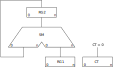
\includegraphics[height = 12\baselineskip]{assets/task-3-01-operation-scheme.pdf}
		\caption{Операційна схема пристрою для обчислення функції~$D$}
		\label{fig:task-3-operation-scheme-01}
		\end{figure}
		
		Розробимо змістовний мікроалгоритм обчислення значення функції. У вихідному стані в регістрах \schel{RG1} і~\schel{RG2} та лічильнику~\schel{CT} знаходяться відповідно операнди $A$, $C$ та~$B$.
		
		Для реалізації множення операнду~$A$ на~$8$ необхідно тричі виконати мікрооперацію зсуву вліво вмісту регістру~\schel{RG1}. Для ділення операнда~$C$ на~$4$ необхідно двічі виконати мікрооперацію зсуву вправо вмісту регістру~\schel{RG2}. Для зменшення на одиницю операнда~$B$ виконується декремент лічильника~\schel{CT}. На етапі обчислення функції у циклі до~\schel{RG2} додається $B - 1$ раз вміст регістру~\schel{RG1}, поданий у доповнювальному коді, тобто реалізуємо мікрооперацію віднімання. Після чого зменшується на одиницю вміст лічильника~\schel{CT}. Обчислення закінчується за виконання умови $CT = 0$. Результат обчислення функції формується в регістрі~\schel{RG2}.
	
		Операція множення виконується четвертим способом. Перед множенням четвертим способом перший множник записуємо у регістр~\schel{RG2}, а другий множник~— в~старші розряди регістру~\schel{RG3} (тобто встановлюємо в~\schel{RG3} значення $Y_0 = Y \cdot 2^{-1}$). У~кожному циклі цифра \schel{RG2}(1), що знаходиться в старшому розряді регістру~\schel{RG2}, керує додаванням, а в \schel{RG3} здійснюється правий зсув на один розряд, що еквівалентно множенню вмісту цього регістра на~$2^{-1}$.
		
		Функціональна схема пристрою для обчислення функції~$D$ зображена на рис.~\ref{fig:task-3-function-scheme}.
		
		\begin{figure}[!htbp]
		\centering
			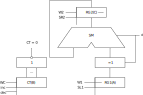
\includegraphics[height = 17\baselineskip]{assets/task-3-02-function-scheme.pdf}
		\caption{Функціональна схема пристрою для обчислення функції~$D$}
		\label{fig:task-3-function-scheme}
		\end{figure}
	\end{solution}
\end{document}